%!TEX root = 2024-cmsb_tool.tex
% Take a model from OdeBase or BioModels.
The functionality described in this section is also available as a Jupyter notebook in \RepoURL.
We introduce a small example to display the functionality of \ToolName.
Suppose we want to study the signaling mechanism in apoptosis as described by kinetic model in~\cite{legewie_mathematical_2006}. 
This model is available in OdeBase under the label \texttt{"BIOMD0000000102"}.

We begin by getting a model from OdeBase:\\
\mintinline{python}{model = ode_scrapper(name="BIOMD0000000102")}\\
To validate the model, we can check its validity via \texttt{model.[attribute]}, where \texttt{attribute} can be the \texttt{name}, \texttt{species}, \texttt{parameters} and \texttt{equations} among others.
Suppose, we want to study the evolution of the observable $C_3$, this corresponds to the variable $x7$ in the model.
To construct an exact lumping that perserves the evolution of $x7$ it suffices to use the following line. \\
\mintinline{python}{exact_lumping = model.lumping([obs_poly])}\\
\ToolName warns us that the exact lumping found is not a reduction as it has the same size as the original one. 

We can use \ToolName to obtain the next reduction, using the following command \\
\mintinline{python}{app_lumping = model.app_lumping([obs_poly])}\\
This command outputs the numerical lumping closest to the exact one. 
Different approximate lumpings can be obtained by providing a value to the \texttt{lumpingTol} keyword argument.
Similarly, we can explore the attributes of the lumped system.
For example, we have that \\
\mintinline{python}{app_lumping.size}\\
Outputs a reduction of size $12$.
This is not a significant reduction. 
To ensure we get a small enough reduction we can use the following command \\
\mintinline{python}{app_lumping = model.app_lumping([obs_poly], max_size=10)}\\
which will output a reduction with a maximum size of $10$.
In this case the computed reduction has a size of $7$.

To see the performance of the approximate lumping we simulate both the original system from 0 to $5000~$seconds using the following lines \\
\mintinline{python}{exact_sim = model.simulate(0, 5000)}\\
A similar line outputs the results for the approximate lumped model. 
The simulations can then be merged using \\
\mintinline{python}{comp_results = merge_simulations(exact_sim, app_sim)}\\
The merged simulation can be immediately plotted by \\
\mintinline{python}{create_figure(comp_results, title=['Original', 'Approximate'])}\\
The resulting plot is show as follows
\begin{figure}
    \centering
    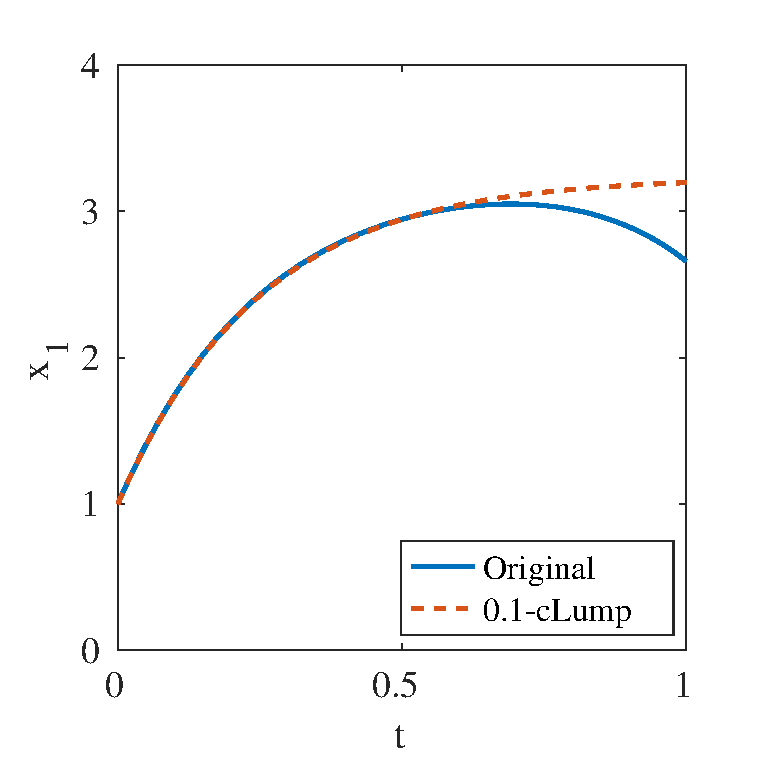
\includegraphics[width=0.3\textwidth]{img/examplecalc.pdf}
    \caption{\comalex{this is a placeholder}
    Time evolution of the $C_3$ concentration using approximate constrained lumping.}
\end{figure}








